\documentclass[12pt, oneside, a4paper]{scrreprt}

\usepackage[manualmark,headsepline,footsepline]{scrlayer-scrpage}

\usepackage[german]{babel}
\usepackage[utf8]{inputenc}
\usepackage{graphicx} %Grafik aktivieren
\usepackage{float}
\usepackage[final]{pdfpages}
\usepackage{hyperref}
\usepackage{pdfcomment}
\usepackage{svg}
\usepackage{csquotes}

\usepackage{siunitx}  
\sisetup{locale = DE,separate-uncertainty}  

\usepackage[backend=biber]{biblatex}
\addbibresource{bib/refs.bib}


%% used for pgfplots, tikzpicture
\usepackage{pgfplots}
\pgfplotsset{compat=newest}

%% the following commands are needed for some matlab2tikz features
\usetikzlibrary{plotmarks}
\usetikzlibrary{arrows.meta}
\usetikzlibrary{datavisualization}
\usetikzlibrary{datavisualization.formats.functions}
\usepgfplotslibrary{patchplots}
\usepackage{array}
\usepackage{grffile} 
\usepackage{amsmath}

\usepackage{todonotes}


\usepackage{listings}
\usepackage{xcolor}

\definecolor{codebg}{HTML}{F5F5F5}
\definecolor{codeframe}{HTML}{D0D0D0}
\definecolor{codekw}{HTML}{0033B3}
\definecolor{codestr}{HTML}{067D17}
\definecolor{codecom}{HTML}{8C8C8C}

\lstdefinestyle{codeblock}{
    language=Python,
    backgroundcolor=\color{codebg},
    frame=single,
    rulecolor=\color{codeframe},
    framesep=4pt,
    framexleftmargin=4pt,
    xleftmargin=4pt,
    xrightmargin=4pt,
    basicstyle=\ttfamily\footnotesize,
    keywordstyle=\color{codekw}\bfseries,
    stringstyle=\color{codestr},
    commentstyle=\color{codecom}\itshape,
    showstringspaces=false,
    breaklines=true,
    breakatwhitespace=true,
    aboveskip=4pt,
    belowskip=4pt,
}
\lstset{style=codeblock}

\usepackage[most]{tcolorbox}


\usepackage[
	format=hang,			% Einstellung fuer Bildunterschriften
%	font={footnotesize},
	font={scriptsize},          % applies to both label and body
%	labelfont={bf,small},  % overrides for the label only ("Figure 3.4")
	textfont={scriptsize},      % overrides for the body only
	labelfont={bf},
	margin=1cm,
	aboveskip=5pt,
	position=bottom
	]{caption}


\pgfplotsset{plot coordinates/math parser=false}
\newlength\fwidth

%%%%%%%%%%%%%%%%%%%%%%%%%%%%%%%%%%%%%%%%%%%%%%%%%%%%%%%%%%%%%%%%%%%%%%%%%%%%%%%%%%%%%%%%%%%%%%%%%%%%%%%%%%%%%%%%%%%%%%%%

%Kapitel-Layout
\usepackage{lmodern} 
%\usepackage{xcolor}
\colorlet{chapter}{black!75}
\addtokomafont{chapter}{\color{chapter}}
\makeatletter% siehe De-TeX-FAQ
\renewcommand*{\chapterformat}{%
    \begingroup% damit \unitlength-Änderung lokal bleibt 
    \setlength{\unitlength}{1mm}% 
    \begin{picture}(20,20)(0,5)% 
    \setlength{\fboxsep}{0pt}% 
    \put(20,20){\line(1,0){\dimexpr 
    \textwidth-20\unitlength\relax\@gobble}}% 
    \put(0,0){\makebox(15,20)[r]{% 
    \fontsize{18\unitlength}{28\unitlength}\selectfont\thechapter 
    \kern-.04em% Ziffer in der Zeichenzelle nach rechts schieben 
    }}% 
    \end{picture} % <-- Leerzeichen ist hier beabsichtigt! 
    \newline
    \endgroup
}

\setlength\parindent{0pt}

%%%%%%%%%%%%%%%%%%%%%%%%%%%%%%%%%%%%%%%%%%%%%%%%%%%%%%%%%%%%%%%%%%%%%%%%%%%%%%%%%%%%%%%%%%%%%%%%%%%%%%%%%%%%%%%%%%%%%%%%

% Kopf- und Fußzeilen, Seitenränder etc.
% Kopf- und Fußzeilen ------------------------------------------------------
\pagestyle{scrheadings}

% Kopf- und Fußzeile auch auf Kapitelanfangsseiten -------------------------
\renewcommand*{\chapterpagestyle}{scrheadings}

% Schriftform der Kopfzeile ------------------------------------------------
\renewcommand{\headfont}{%
\normalfont
}

% Kopfzeile ----------------------------------------------------------------
\ihead{Regelungstechnisches Praktikum (RTP)}
\chead{}
\ohead{
\includegraphics[width=0.3\textwidth]{figure/oth-regensburg-logo}}
%
\setlength{\headheight}{21mm} % Höhe der Kopfzeile
%\setheadsepline[text]{0.4pt} % Trennlinie unter Kopfzeile

% Fußzeile -----------------------------------------------------------------
\ifoot{Marius Off, Janis Graf}
\cfoot{\today}
\ofoot{\pagemark}


% erzeugt ein wenig mehr Platz hinter einem Punkt --------------------------
\frenchspacing 

\clubpenalty = 10000
\widowpenalty = 10000 
\displaywidowpenalty = 10000


\newcommand{\mt}[1]{\textrm{#1}}



%%%%%%%%%%%%%%%%%%%%%%%%%%%%%%%%%%%%%%%%%%%%%%%%%%%%%%%%%%%%%%%%%%%%%%%%%%%%%%%%%%%%%%%%%%%%%%%%%%%%%%%%%%%%%%%%%%%%%%%%
%%%%%%%%%%%%%%%%%%%%%%%%%%%%%%%%%%%%%%%%%%%%%%%%%%%%%%%%%%%%%%%%%%%%%%%%%%%%%%%%%%%%%%%%%%%%%%%%%%%%%%%%%%%%%%%%%%%%%%%%
%%%%%%%%%%%%%%%%%%%%%%%%%%%%%%%%%%%%%%%%%%%%%%%%%%%%%%%%%%%%%%%%%%%%%%%%%%%%%%%%%%%%%%%%%%%%%%%%%%%%%%%%%%%%%%%%%%%%%%%%

\begin{document}
    % \todototoc
    % \listoftodos

    \begin{titlepage}

        \begin{tabular}{l r} 
            
\includegraphics[width=0.5\textwidth]{figure/oth-regensburg-logo.jpg}
            &
        \end{tabular}
        \vspace{1cm}

        \begin{minipage} [c] [8.5cm] [b] {\textwidth}
            \Huge{
                \begin{center}
                    \textbf{Praktikum Regelungstechnik (RTP)}\\[0.8cm]
                    \textbf{Versuch T4:\\RetBot system identification, part II} \\[1.5cm]
                    \par
                    %{\large Versuch 3}\\[1cm]
                    {\large \today} \\[1cm]
                \end{center}
                }
        \end{minipage}

        \vspace{0.1cm}

        \begin{minipage} [c] [3.5cm] [b] {\textwidth}
            \begin{center}
                \vspace{0.3cm}
                Gruppe 38\\
                Marius Off\\
                Janis Graf\\
                \vspace{0.5cm}
                %\texttt{Dokument-Version: 02}\\
            \end{center}
        \end{minipage}

    \end{titlepage}

    \tableofcontents


    \chapter{Preparations}\label{chap:preperations}

        \section{(aV) Steps to solve the control task}
            In order to solve a control problem, a mathematical model of the controlled system is first developed and the performance requirements of the control system are defined. The controller is then designed based on this, during which the structure and parameters of the control law are specified. Finally, the controller is implemented in hardware or software and validated on the actual system. This process is illustrated in Figure \ref{fig:loesungsweg_lunze} according to Lunze~\cite{Lunze2016}.

            \begin{figure}[H]
                \centering
                \begin{tikzpicture}[>=stealth, line width=0.8pt, scale=0.8, node distance=2.8cm]
                    
                    % Knoten
                    \node (g) {Controlled system, quality requirements};
                    \node[below=of g] (model) {Model of the controlled system and performance requirements};
                    \node[below=of model] (law) {Controller law};
                    \node[below=of law] (ctrl) {Controller};
                    \draw[->] (g) -- (model)
                    node[midway, right=0.4cm] {\textit{Modeling}};
                    \draw[->] (model) -- (law)
                    node[midway, right=0.4cm] {\textit{Controller Design}};
                    \draw[->] (law) -- (ctrl)
                    node[midway, right=0.4cm] {\textit{Implementation}};
                    
                \end{tikzpicture}
                \caption{Approach to control engineering problems according to Lunze~\cite{Lunze2016}}
                \label{fig:loesungsweg_lunze}
            \end{figure}

            \cleardoubleemptypage

        \section{(bV) Block diagram of the control loop}
            
            \begin{figure}[H]
                \centering
                \begin{tikzpicture}[>=stealth, line width=0.8pt,
                    scale=0.7, every node/.style={transform shape}]
                    
                    %--- Blöcke -------------------------------------------------------------
                    \node[draw, minimum width=4cm, minimum height=3cm] (motor) {};
                    \node[draw, minimum width=4cm, minimum height=3cm, right=2.5cm of motor] (drive) {};
                    \node[draw, minimum width=4cm, minimum height=3cm, right=2.5cm of drive] (kin) {};
                    
                    %--- Beschriftungen oberhalb der Blöcke --------------------------------
                    \node[above=4pt of motor.north] {$K_{P1} \quad T_1$};
                    \node[above=4pt of drive.north] {$K_{P2}$};
                    \node[above=4pt of kin.north] {$K_I$};
                    
                    %--- Beschriftungen unterhalb der Blöcke --------------------------------
                    \node[below=4pt of motor.south] {Motor (PT$_1$ element)};
                    \node[below=4pt of drive.south] {Drive (P-element)};
                    \node[below=4pt of kin.south] {Kinematics (I-element)};
                    
                    %--- Verbindungs-Pfeile mit Signalbezeichnungen -------------------------
                    \draw[->] ($(motor.west)+(-2.0,0)$) -- (motor.west)
                    node[midway, above] {$\delta_\text{Mot} \,/\, \%$};
                    
                    \draw[->] (motor.east) -- (drive.west)
                    node[midway, above] {$\omega \,/\, \mathrm{rad/s}$};
                    
                    \draw[->] (drive.east) -- (kin.west)
                    node[midway, above] {$v_\text{EV3} \,/\, \mathrm{cm/s}$};
                    
                    \draw[->] (kin.east) -- ($(kin.east)+(2.0,0)$)
                    node[midway, above] {$x_\text{EV3} \,/\, \mathrm{cm}$};
                    
                    %-----------------------------------------------------------------------
                    % Innenleben der Blöcke: Kennlinien (schematisch)
                    %-----------------------------------------------------------------------
                    
                    % Motorblock: PT1-ähnliche Sprungantwort
                    \path (motor.south west) ++(0.5,0.5) coordinate (mO);
                    \draw (mO) -- ++(0,2.0);
                    \draw (mO) -- ++(2.6,0);
                    \draw (mO)
                    .. controls ++(0.4,1.2) and ++(-0.6,0.0) ..
                    ++(1.4,1.8) -- ++(0.8,0);
                    
                    % Antriebsblock: P-Glied
                    \path (drive.south west) ++(0.5,0.5) coordinate (dO);
                    \draw (dO) -- ++(0,2.0);
                    \draw (dO) -- ++(2.6,0);
                    \draw ($(dO)+(0.0,1.3)$) -- ++(2.6,0);
                    
                    % Kinematikblock: I-Glied
                    \path (kin.south west) ++(0.5,0.5) coordinate (kO);
                    \draw (kO) -- ++(0,2.0);
                    \draw (kO) -- ++(2.6,0);
                    \draw (kO) -- ++(2.3,1.7);
                    
                \end{tikzpicture}
                \caption{The block diagram illustrates the configuration of the EV3 robot.}
                \label{fig:ev3_blockdiagramm}
            \end{figure}

        The control process of the EV3 robot (Figure \ref{fig:ev3_blockdiagramm}) begins with the duty cycle $\delta$, which is provided as an input signal in the form of pulse width modulation (PWM). This signal determines the average voltage of the DC motor and, consequently, the torque and rotational speed. The resulting rotational speed is transmitted to the wheels via the gearbox and converted into the robot's linear translational speed. Finally, the robot's kinematics describe the relationship between the rotational movements of the individual wheels and the resulting overall movement of the robot.


        \section{(cV) Block diagram of a distance control system (according to DIN IEC 60050-351).}\label{sec:cV}

            Diagram \ref{fig:distance_control_block_diagram} shows a block diagram of a distance control system using a P controller according to DIN IEC 60050-351~\cite{DIN_IEC_60050-351_2014}. The system consists of a reference variable $w$ (target distance), a control difference $e$, a manipulated variable $y$, an initial distance $x_0$, a controlled variable $x$ (actual distance), and a feedback variable $r$. The controlling element processes the control difference to generate the manipulated variable $y$ acting on the controlled system. The controlled system produces the travelled distance $x_\mathrm{traveled}$, which is subtracted from the initial distance $x_0$ at a summing junction to yield the actual distance $x = x_0 - x_\mathrm{traveled}$; the measuring element then provides the feedback variable $r$ from this controlled variable.

            \begin{figure}[H]
                \centering
                \begin{tikzpicture}[
                        auto,
                        >=stealth,
                        line width=0.7pt,
                        scale=0.78,
                        transform shape,
                        node distance=2.4cm,
                        block/.style={
                                draw,
                                rectangle,
                                minimum height=2.4em,
                                minimum width=4.5em,
                                align=center,
                                font = {\scriptsize}
                            },
                        sum/.style={
                                draw,
                                circle,
                                minimum size=0.6cm,
                                inner sep=0pt
                            },
                        input/.style={coordinate},
                        output/.style={coordinate},
                        pinstyle/.style={pin edge={to-,thin,black}}
                    ]

                    % --- Forward path nodes -------------------------------------------
                    \node [input, name=input] {};
                    \node [sum, right of=input]                       (sum)   {};
                    \node [block, right of=sum]                       (ctrl)  {Controlling element\\ ($K_\mathrm{P}$)\\ \emph{(Reglerglied)}};
                    \node [block, right of=ctrl, node distance=3.6cm]
                    (plant) {Controlled system\\ ($K_\mathrm{I}$)\\ (vehicle drive)\\ \emph{(Regelstrecke)}};
                    % initial-distance summing node on the x-line
                    \node [sum, right of=plant, node distance=3.4cm] (xsum) {};
                    \node [output, right of=xsum, node distance=2.4cm] (output) {};

                    % --- Initial distance into the summing node ----------------------------
                    \node [above of=xsum, node distance=1.8cm] (init) {$x_0$ (\emph{Anfangsabstand})};
                    \draw [->] (init) -- node[pos=0.75, right] {\small $+$} (xsum);

                    % --- Travelled distance into the summing node -----------
                    \draw [->] (plant) -- node[pos=0.5] {$x_\mathrm{traveled}$} node[pos=0.88, below] {\small $-$} (xsum);

                    % --- Measuring element in the feedback path (centred) -------------
                    \node [block, below of=plant, node distance=2.8cm]
                    (sensor)
                    {Measuring element\\ (odometry)\\ \emph{(Messglied)}};

                    % --- Forward connections ------------------------------------------
                    \draw [->] (input) -- node {$w$} (sum);
                    \draw [->] (sum)   -- node {$e$} (ctrl);
                    \draw [->] (ctrl)  -- node[pos=0.5] {$y$} (plant);
                    \draw [->] (xsum)  -- node [name=x] {$x$} (output);

                    % --- Feedback connections -----------------------------------------
                    \coordinate (tap) at ($(xsum)!0.55!(output)$);
                    \node[circle, fill, inner sep=1.2pt] at (tap) {};
                    \draw [->] (tap) |- (sensor.east);
                    \draw [->] (sensor.west) -| node[pos=0.99] {$-$}
                    node[near end] {$r$} (sum);

                    % --- Sign of the reference input at the summing junction ----------
                    \node at ([shift={(-0.30cm,0.18cm)}]sum.north west) {\small $+$};

                    % --- Legend (DIN IEC 60050-351 designations) ----------------------
                    \node[align=left, font=\footnotesize, anchor=north west]
                    at (sensor.south -| input |- sensor.south) [yshift=-0.8cm]
                    {%
                        $w$: reference variable (\emph{Führungsgröße}, target distance)\\
                        $e$: control difference (\emph{Regeldifferenz}), $e = w - r$\\
                        $y$: manipulated variable (\emph{Stellgröße})\\
                        $x_0$: initial distance (\emph{Anfangsabstand})\\
                        $x_\mathrm{traveled}$: travelled distance (\emph{zurückgelegte Strecke})\\
                        $x$: controlled variable (\emph{Regelgröße}, actual distance)\\
                        $r$: feedback variable (\emph{Rückführgröße})%
                    };

                \end{tikzpicture}
                \caption{Block diagram of a distance control system using a P controller according to DIN IEC 60050-351}
                \label{fig:distance_control_block_diagram}
            \end{figure}

%%%%%%%%%%%%%%%%%%%%%%%%%%%%%%%%%%%%%%%%%%%%%%%%%%%%%%%%%%%%%%%%%%%%%%%%%%%%%%%%%%%%%%%%%%%%%%%%%%%%

    \chapter{Experiment T4: RetBot system identification, part 2}\label{ch:ExperimentT4}
        \section{(d) System description}\label{sec:d-system-description}

            \begin{displaycquote}{RTP_Versuche}
                \footnotesize{\textit{(d) Use the recorded data from the previous experiment and write a Matlab program that calculates the data required for the system description for both the left and right drives. Draw graphs containing the four different conditions and the tangents, ... you applied for determining the system behavior. Consider a reasonable time frame, rather than adopting a ``take what's available'' approach.}} 
            \end{displaycquote}\label{task(d)}

            Each drive train is modelled as an IT$_1$ element with the transfer function $G(s) = K_I / [\,s\,(T_1\,s + 1)\,]$, mapping the input duty cycle $\delta\,/\,\%$ to the traveled distance $x\,/\,\mathrm{cm}$ of the wheel. The two parameters --- the integral gain $K_I$ and the time constant $T_1$ --- are extracted from the recorded step responses by an asymptotic-tangent procedure, carried out separately for the left wheel (QEI1) and the right wheel (QEI2) at each of the four duty cycles $\delta \in \{25,\,50,\,75,\,100\}\,\%$.

            The QEI step counts are first converted into a traveled distance via the wheel circumference,
            \begin{equation}
                x = \frac{\text{steps}}{360^\circ} \cdot d_R \cdot \pi, \qquad d_R = \SI{5.6}{\cm},
                \label{eq:weg_aus_winkel}
            \end{equation}
            where one encoder revolution ($360^\circ$) advances the wheel by its circumference $d_R\,\pi$.

            For each step response $x(t)$, the asymptotic tangent $x_\infty(t) = a\,t + b$ is fitted by linear regression to the settled (linear) tail of the recording. Because the IT$_1$ step response asymptotically approaches the ramp $K_I\,\delta\,(t - T_1)$, the tangent slope yields the integral gain normalised per duty-cycle percentage,
            \begin{equation}
                K_I = \frac{a}{\delta},
            \end{equation}
            and its time-axis intersection yields the time constant,
            \begin{equation}
                T_1 = -\frac{b}{a} - t_\text{step},
            \end{equation}
            where $t_\text{step}$ denotes the instant at which the duty cycle is applied. The four per-duty-cycle estimates are then averaged for each motor (Figures~\ref{fig:QEI_left} and \ref{fig:QEI_right}), giving the operating-point-independent parameters $\overline{K_I}$ and $\overline{T_1}$ that enter the differential equations in Section~\ref{sec:e-differential-equations}.

            \begin{figure}[H]
                \centering
                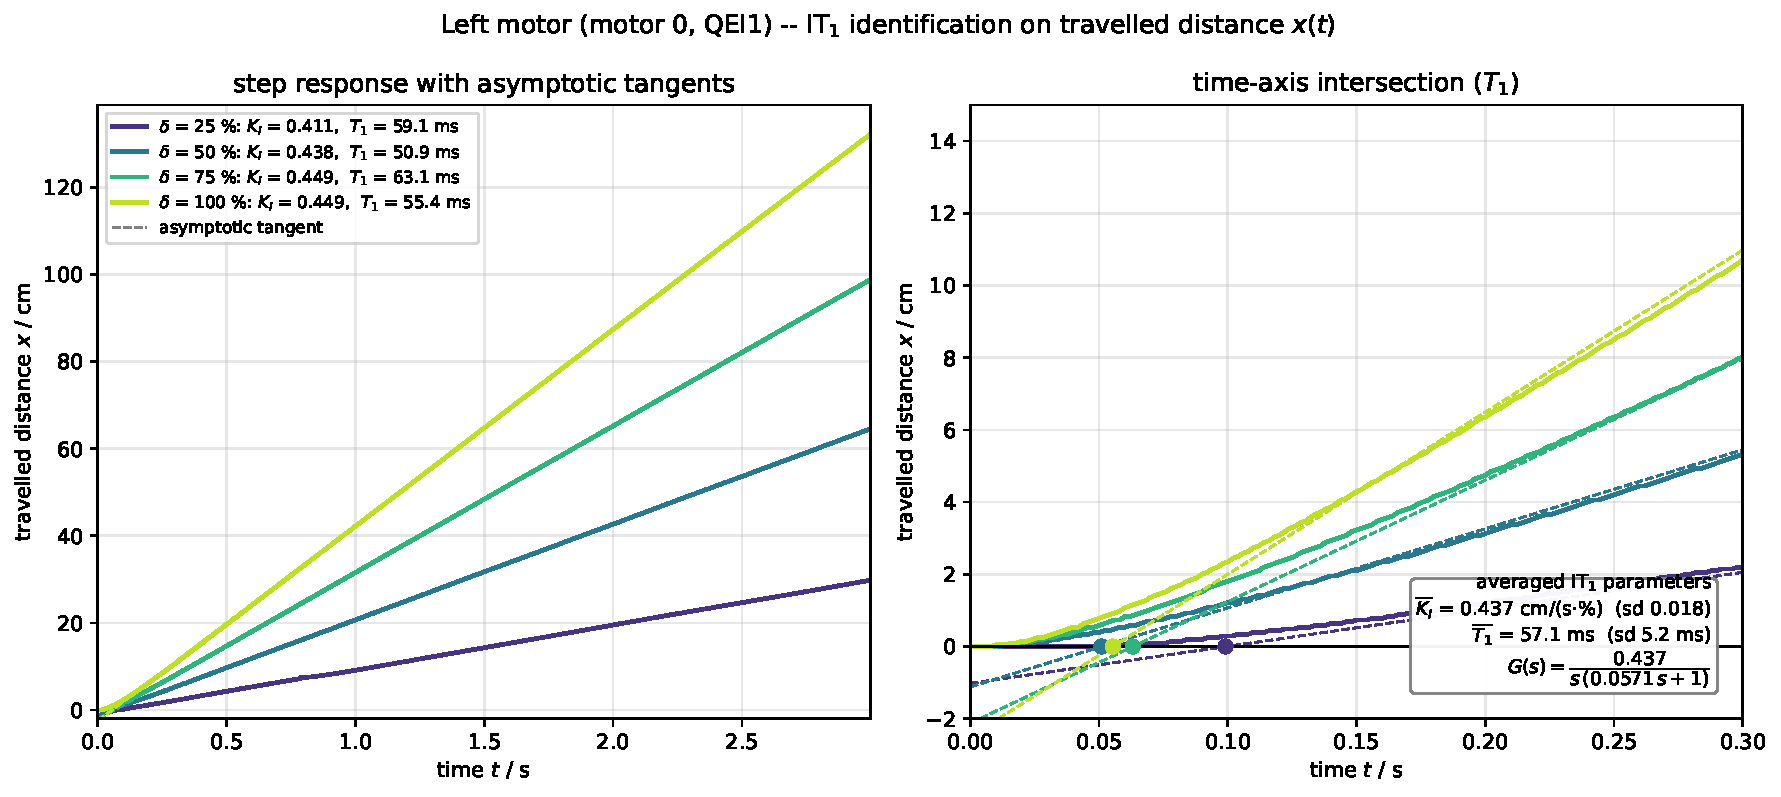
\includegraphics[width=\textwidth]{figure/it1-distance-left.pdf}
                \caption{Left drive (motor 0, QEI1): traveled distance $x(t)$ for all four duty cycles together with the fitted asymptotic tangents. Per-duty-cycle values of $K_I$ and $T_1$ are given in the legend; the right panel zooms onto the time-axis intersections that yield $T_1$ and shows the averaged IT$_1$ parameters $\overline{K_I}$, $\overline{T_1}$, and the resulting transfer function $G(s)$.}
                \label{fig:QEI_left}
            \end{figure}

            \begin{figure}[H]
                \centering
                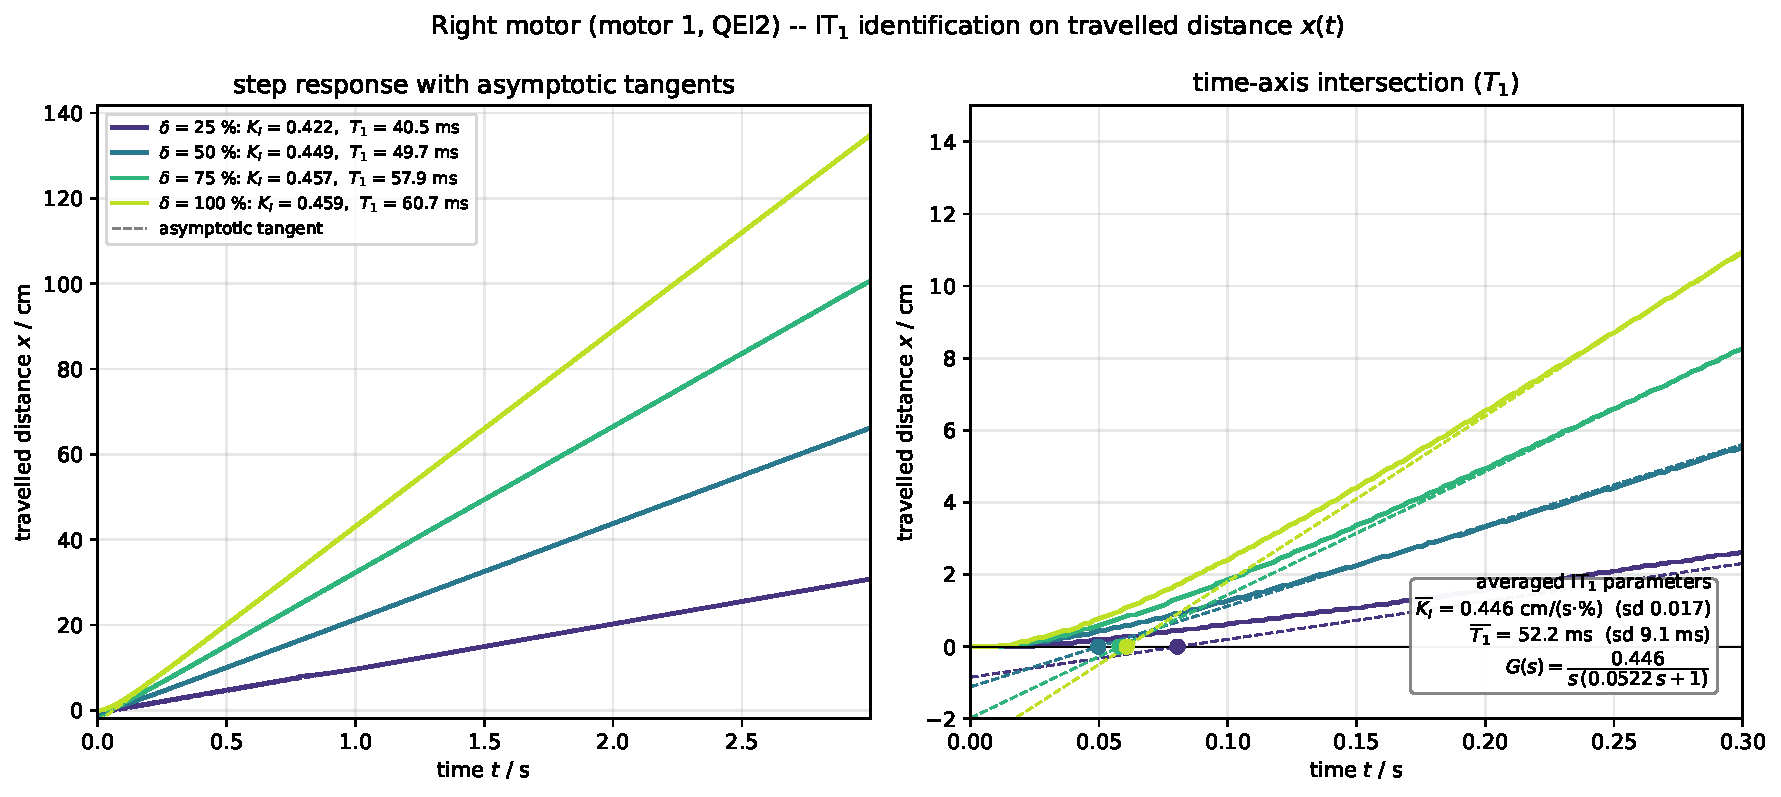
\includegraphics[width=\textwidth]{figure/it1-distance-right.pdf}
                \caption{Right drive (motor 1, QEI2): traveled distance $x(t)$ for all four duty cycles together with the fitted asymptotic tangents. Per-duty-cycle values of $K_I$ and $T_1$ are given in the legend; the right panel zooms onto the time-axis intersections that yield $T_1$ and shows the averaged IT$_1$ parameters $\overline{K_I}$, $\overline{T_1}$, and the resulting transfer function $G(s)$.}
                \label{fig:QEI_right}
            \end{figure}

            \subsection{Resulting Parameters}

            The per-duty-cycle results and their averages are summarised in Listing~\ref{lst:it1-params}. The integral gain is consistent across duty cycles --- the relative standard deviation stays below \qty{5}{\percent} for both motors --- which confirms the validity of the IT$_1$ structure within the considered operating range. The time constants scatter more strongly (up to $\sigma_{T_1} \approx \qty{9}{\milli\second}$ on the right drive), reflecting the higher sensitivity of $T_1$ to encoder quantisation at low duty cycles, where the resolution of one QEI step ($\approx \qty{0.049}{\centi\metre}$) is appreciable relative to the slow rise of the response. The same effect produces the small initial offset visible in both \qty{25}{\percent} traces; it does not bias the identification because only the linear tail of the recording enters the tangent regression.

            The two drives behave near-symmetrically: their averaged integral gains $\overline{K_{I,L}} = \qty{0.437}{\centi\metre\per\second\per\percent}$ and $\overline{K_{I,R}} = \qty{0.446}{\centi\metre\per\second\per\percent}$ agree within one standard deviation, and their time constants differ by less than \qty{5}{\milli\second}. The averaged parameters $\overline{K_I}$ and $\overline{T_1}$ obtained here are used directly in the differential equations and transfer functions of Section~\ref{sec:e-differential-equations}.

            \begin{lstlisting}[caption={Identified IT$_1$ parameters per duty cycle and averaged values for the left and right drive.},label={lst:it1-params}]
motor drive   delta/%  slope_inf/cm/s  K_I/cm/(s*%)    T_1/ms
Left motor (motor 0, QEI1)  25 %   25.0000         10.2724        0.4109   59.1133
Left motor (motor 0, QEI1)  50 %   50.0000         21.8954        0.4379   50.9466
Left motor (motor 0, QEI1)  75 %   75.0000         33.6763        0.4490   63.0547
Left motor (motor 0, QEI1) 100 %  100.0000         44.9191        0.4492   55.3605
Right motor (motor 1, QEI2)  25 %   25.0000         10.5382        0.4215   40.4807
Right motor (motor 1, QEI2)  50 %   50.0000         22.4389        0.4488   49.6909
Right motor (motor 1, QEI2)  75 %   75.0000         34.2385        0.4565   57.9448
Right motor (motor 1, QEI2) 100 %  100.0000         45.8991        0.4590   60.7124

Left motor (motor 0, QEI1)
    K_I_avg = 0.4368 cm/(s*%)   (sd 0.0180)
    T_1_avg = 57.12 ms = 0.0571 s   (sd 5.18 ms)
    G(s) = 0.437 / (s (0.0571 s + 1))

Right motor (motor 1, QEI2)
    K_I_avg = 0.4465 cm/(s*%)   (sd 0.0172)
    T_1_avg = 52.21 ms = 0.0522 s   (sd 9.11 ms)
    G(s) = 0.446 / (s (0.0522 s + 1))
            \end{lstlisting}

            \cleardoubleemptypage

        \section{(e) Differential equations and transfer functions for both drives.}\label{sec:e-differential-equations}

            \begin{displaycquote}{RTP_Versuche}
                \footnotesize{\textit{(e) Specify the descriptive differential equations and transfer functions for both the left and right drives (note: average value across the different duty cycles). Compare the step response of the identified system with the measured data to identify any inconsistencies.}}
            \end{displaycquote}\label{task(e)}

            The following paragraphs describe the differential equations and transfer functions for both the left and right drives using constants from the previous section.

            The differential equation for an IT$_1$ system is given by:
            \begin{equation}
                T_1 \dot{x}(t) + x(t) = K_I \int x_e(t) \, dt
            \end{equation}

            The transfer function for an IT$_1$ system is given by:
            \begin{equation}
                G(s) = \frac{K_I}{s(T_1 s + 1)} 
            \end{equation}


            \subsection{Left Motor}\label{subsec:left-motor}

            The parameters of the left drive (motor~0, QEI1) were identified individually for each of the four duty cycles and then averaged. The integral gain $K_I$ was obtained from the slope of the asymptotic tangent (normalised per duty-cycle percentage), and the time constant $T_1$ from the intersection of that tangent with the time axis.

            For the left motor, the averaged parameters are given by Figure \ref{fig:QEI_left}:

            \begin{equation}
                K_{I,L} = \qty{0.437}{\centi\metre\per\second\per\percent}, \qquad
                T_{1,L} = \qty{57.1}{\milli\second} = \qty{0.0571}{\second}
            \end{equation}

            This yields the differential equation for the velocity $v_L(t)$:

            \begin{equation}
                T_{1,L}\,\dot{v}_L(t) + v_L(t) = K_{I,L}\,\delta_L(t)
                \quad\Rightarrow\quad
                \qty{0.0571}{\second}\,\dot{v}_L(t) + v_L(t) = \qty{0.437}{\centi\metre\per\second\per\percent}\,\delta_L(t)
            \end{equation}

            The corresponding transfer function $G_L(s)$ is:

            \begin{equation}
                G_L(s) = \frac{K_{I,L}}{s\,(T_{1,L}\,s + 1)} = \frac{0.437}{s\,(0.0571\,s + 1)}
            \end{equation}


            \subsection{Right Motor}\label{subsec:right-motor}

            The parameters of the right drive (motor~1, QEI2) were identified using the same procedure as for the left drive: $K_I$ from the normalised asymptotic-tangent slope and $T_1$ from its time-axis intersection, averaged over the four duty cycles.

            For the right motor, the averaged parameters are given by Figure \ref{fig:QEI_right}:

            \begin{equation}
                K_{I,R} = \qty{0.446}{\centi\metre\per\second\per\percent}, \qquad
                T_{1,R} = \qty{52.2}{\milli\second} = \qty{0.0522}{\second}
            \end{equation}

            This yields the differential equation for the velocity $v_R(t)$:

            \begin{equation}
                T_{1,R}\,\dot{v}_R(t) + v_R(t) = K_{I,R}\,\delta_R(t)
                \quad\Rightarrow\quad
                \qty{0.0522}{\second}\,\dot{v}_R(t) + v_R(t) = \qty{0.446}{\centi\metre\per\second\per\percent}\,\delta_R(t)
            \end{equation}

            The corresponding transfer function $G_R(s)$ is:

            \begin{equation}
                G_R(s) = \frac{K_{I,R}}{s\,(T_{1,R}\,s + 1)} = \frac{0.446}{s\,(0.0522\,s + 1)}
            \end{equation}




            \cleardoubleemptypage

        \section{(f) Simulink simulation of the control loop}\label{sec:f-simulink-simulation}


            \begin{displaycquote}{RTP_Versuche}
                \footnotesize{\textit{(f) Create a Simulink simulation of the control loop designed in the preparation phase for the distance control using the identified system as the plant and a P controller. Use a gain $KP = \qty{-10}{\percent\per\cm}$, a target distance of \qty{25}{\cm} and an initial distance of \qty{80}{\cm} for testing. Use the integration method ode3 (Bogacki-Shampine) with a fixed step size of \qty{20}{\ms}. Do not forget the rate-limit-block (see 3.7) and use a value of $\frac{\qty{4}{\percent}}{20\,\text{ms}}$.
                \vspace{2mm}\\
                Plot the reference variable, the manipulated variable and the controlled variable.
                \vspace{2mm}\\
                What does this sampling time mean in terms of control engineering?\\
                Which nonlinear element do you also need to add to the simulation to simulate real conditions?}}
            \end{displaycquote}\label{task(f)}

            The distance-control loop of Section~\ref{sec:cV} is implemented in Simulink with the two identified IT$_1$ plants of Section~\ref{sec:e-differential-equations}; the model is shown in Figure~\ref{fig:simulink_control_loop}. The P controller uses $K_P = \qty{-10}{\percent\per\centi\metre}$ --- negative because the measurement convention $x = x_0 - x_\text{traveled}$ adopted in Section~\ref{sec:cV} makes the controlled variable decrease as the robot moves towards the target. The rate-limit block bounds $|\dot{\delta}| \le \qty{4}{\percent}/\qty{20}{\milli\second}$, and integration is fixed-step \texttt{ode3} (Bogacki--Shampine) with $T_s = \qty{20}{\milli\second}$, reference $w = \qty{25}{\centi\metre}$, and initial distance $x_0 = \qty{80}{\centi\metre}$.

            \begin{figure}[H]
                \centering
                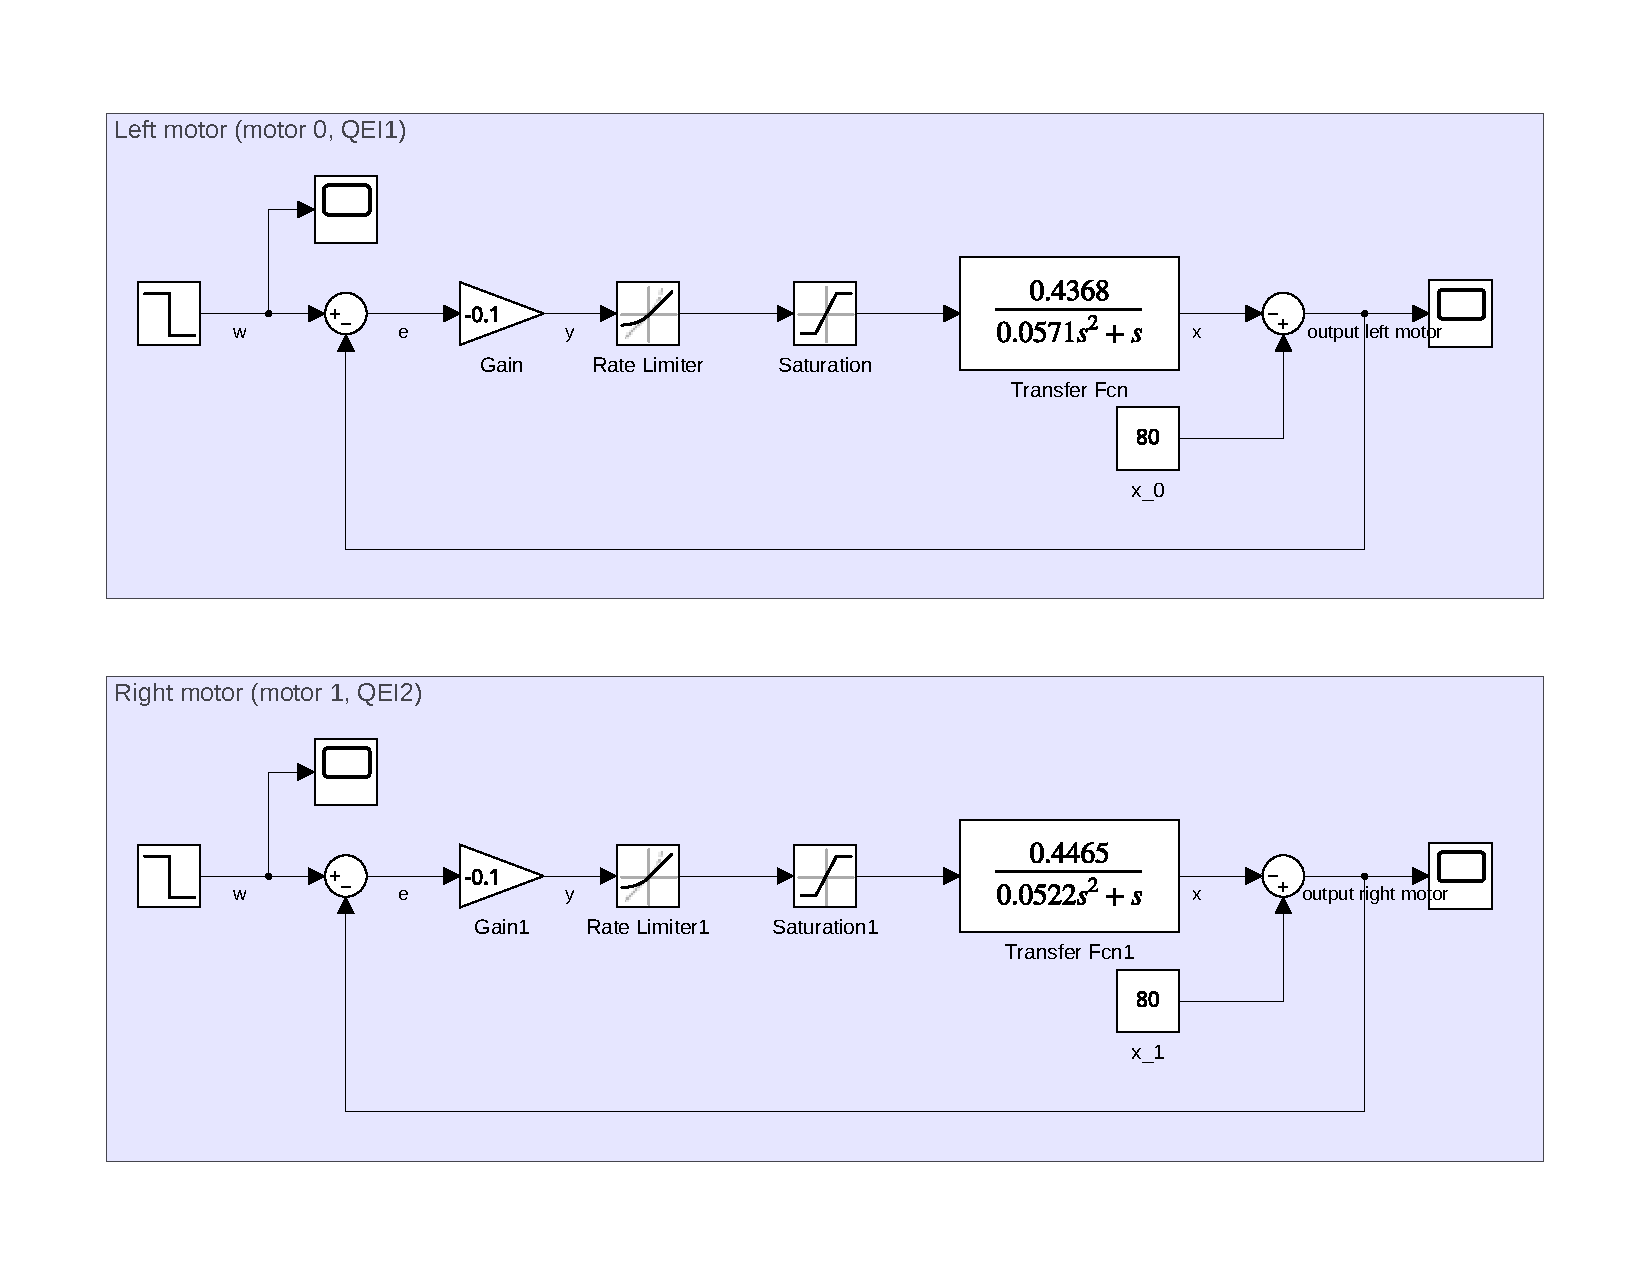
\includegraphics[width=\textwidth]{figure/simulink_system.pdf}
                \caption{Simulink model of the distance control loop with the identified IT$_1$ plants for both drives.}
                \label{fig:simulink_control_loop}
            \end{figure}

            Figure~\ref{fig:simulink_output} shows the simulated reference $w$ and controlled variable $x$ for both drives. Starting from $x_0 = \qty{80}{\centi\metre}$, $x$ decreases monotonically toward the target $w = \qty{25}{\centi\metre}$ without overshoot, and the two drive trains track each other to within plotting accuracy. The transient is shaped by the combination of the rate-limited manipulated variable and the dominant time constant of the IT$_1$ plant; the steady-state error converges to zero because the plant's integrator pole supplies the type-1 behaviour the pure P controller cannot provide on its own.

            \begin{figure}[H]
                \centering
                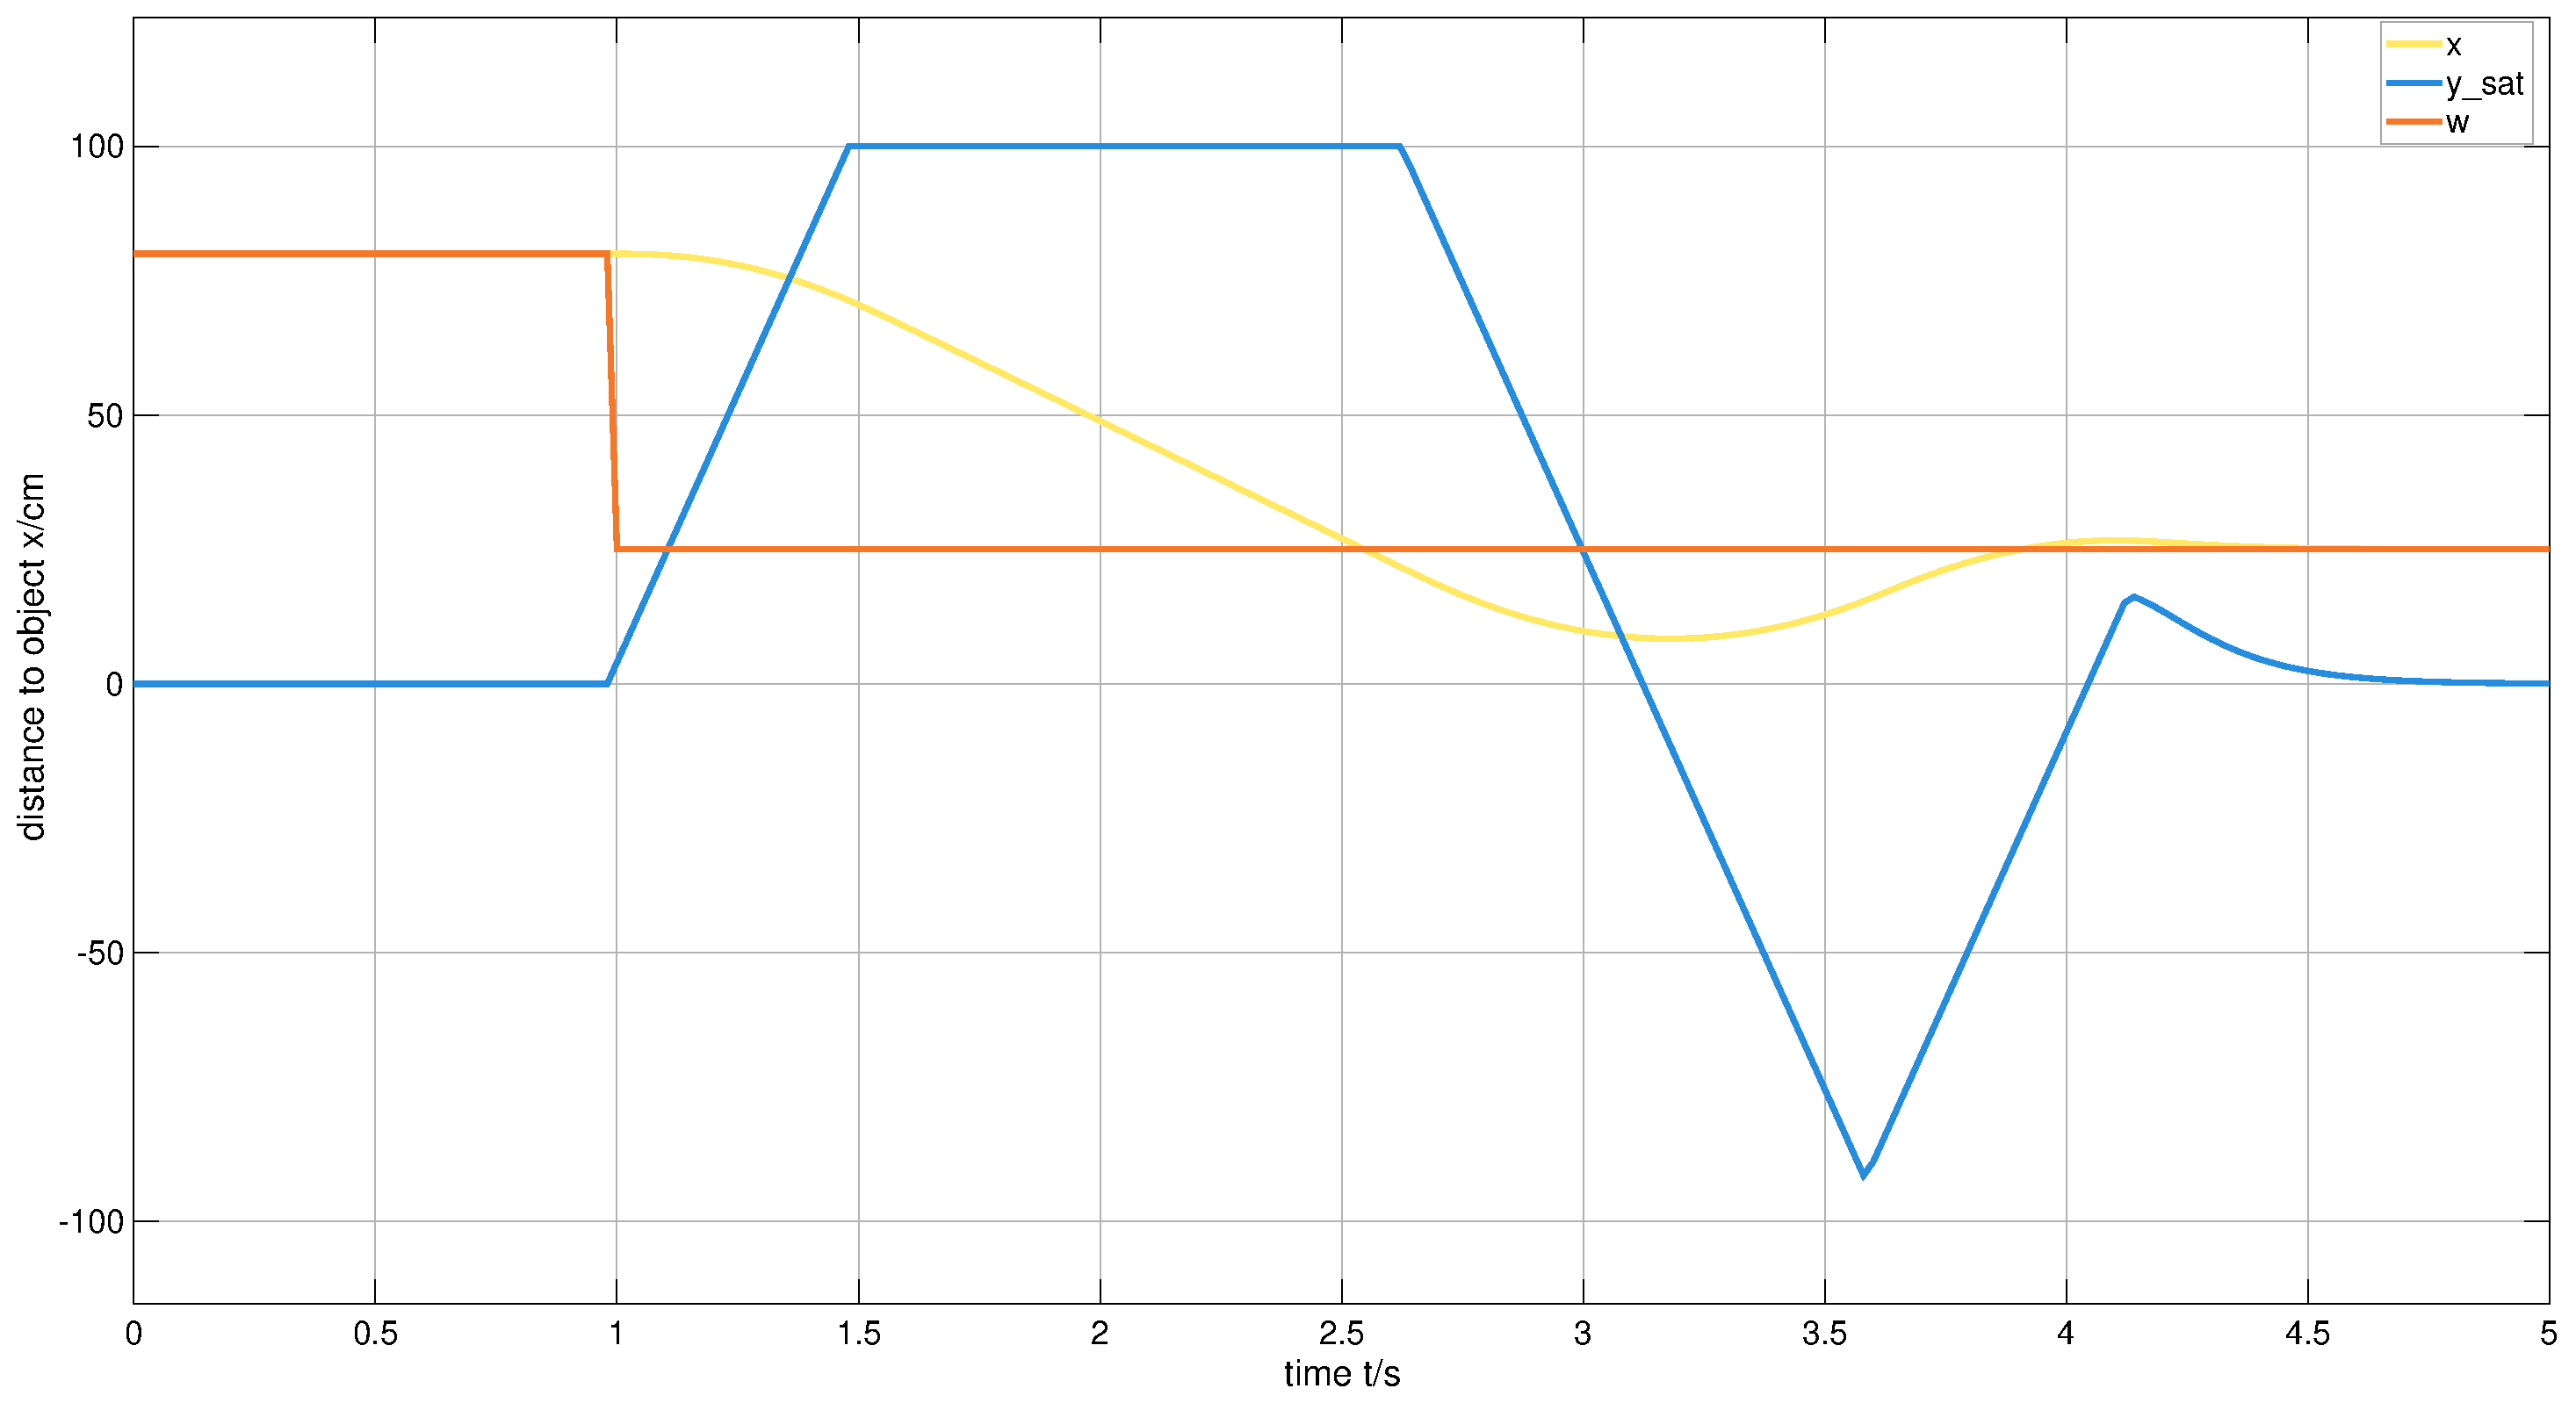
\includegraphics[width=0.6\textwidth]{figure/RTP-system-output.eps}
                \caption{Simulink output: reference $w$ and controlled variable $x$ for the left and right drive.}
                \label{fig:simulink_output}
            \end{figure}

            \paragraph{Sampling time.}
            The fixed step $T_s = \qty{20}{\milli\second}$ corresponds to a sampling rate $f_s = \qty{50}{\hertz}$ and a Nyquist frequency of \qty{25}{\hertz}. Relative to the dominant plant time constant $T_1 \approx \qty{55}{\milli\second}$ this yields $T_1 / T_s \approx 3$, below the common digital-control guideline $T_1 / T_s \ge 10$. The loop remains stable for the values used here, but the coarse discretisation visibly limits how finely the rate-limited manipulated variable can track the desired control law and would degrade disturbance rejection at higher frequencies. In control-engineering terms, the interval between two sampling instants acts practically as a \emph{dead time} (\emph{Totzeit}): the zero-order hold keeps the manipulated variable constant between updates and the controller responds only at the next step, so a change is answered up to one sampling period $T_s$ late (about $T_s/2$ on average). This effective dead time introduces additional phase lag and therefore reduces the available phase margin.

            \paragraph{Required non-linearity.}
            A \emph{saturation} block on the manipulated variable, clipping $\delta$ to the physically realisable PWM range $\pm \qty{100}{\percent}$, must be added to reflect the EV3 hardware. Without it the linear P controller demands $\delta = K_P\,(w - x_0) = \qty{550}{\percent}$ at the moment of the step --- a value the drive cannot produce, so the simulation would overestimate the achievable closing speed of the real system.





            \cleardoublepage







    \appendix
        % \makeatletter
        
    \chapter{Appendix Frontmatter}

        \section{Declarations}\label{app:statutory}

            \begin{enumerate}
                \item Wir erklären hiermit, dass wir dieses Dokument selbstständig verfasst, noch nicht anderweitig für Prüfungszwecke vorgelegt, keine anderen als die angegebenen Quellen und Hilfsmittel benutzt sowie wörtliche und sinngemäße Zitate als solche gekennzeichnet haben.
            \end{enumerate}

            \vskip22mm
            Regensburg, den 2026-05-01, \\
            "\hskip6cm Marius Off\hskip2cm Matrikelnummer:~3416002,\\
            "\hskip6cm Janis Graf\hskip2cm Matrikelnummer:~3377251
            \vskip1mm
            \hrule
            \vskip1mm
            {\footnotesize Ort, Datum und Unterschrift}

            \vspace{12mm}

            \cleardoublepage

        \listoffigures

        %\listoftables

            \cleardoublepage

    \chapter{Appendix Code and Resources}



            \section{Code used for the analysis of the Preperations}
            
            %\lstinputlisting[caption={Code used for the analysis of the Preperations}, label={lst:preperations}]{../02_Preperations/RTP-T2-analysis.ipynb}

                \begin{tcolorbox}[
                    colback=red!10,
                    colframe=red!70!black,
                    title=\textbf{Editorial note — Source code omitted},
                    fonttitle=\bfseries,
                    sharp corners=south,
                ]
                    The full source code for the analysis (a Jupyter notebook of this time approximately 1{,}500 lines and a simulink model) is \textbf{\emph{not}} included in this appendix. Including it as a verbatim listing caused major build instability again and was therefore deliberately omitted.

                    The complete source can be obtained by either of the following means:
                    \begin{itemize}
                        \item By email request to \texttt{janis.graf@st.oth-regensburg.de}
                        \item Via requesting access to the GitHub repository: \url{https://github.com/janisgra/RTP-T4-SoSe2026.git}
                    \end{itemize}
                \end{tcolorbox}
        
        %%%%%%%%%%%%%%%%%%%%%%%%%%%%%%%%%%%%%%%%%%%%%%%%%%%%%%%%%%%%%%%%%%%%%
        %\chapter{Bibliography}
        %%%Literaturverzeichnis
        \printbibliography

        %%%%%%%%%%%%%%%%%%%%%%%%%%%%%%%%%%%%%%%%%%%%%%%%%%%%%%%%%%%%%%%%%%%%%

\end{document}